First of all, before even thinking about programming language, we had to think of a solid and re-usable architecture for
our application. Because we had to build a GUI that would launch openMVG executable, we quickly choose to use the 
model/view/controller pattern. This pattern is pretty simple to understand : the user uses a controller which will manipulate
the model which will update the view that the user sees. In our context, the model correspond to the openMVG executables for example. 
What we actually choose was to modify a bit this pattern to perfectly fit our needs : we would merge the controller and view
together, we will explain later why.

Once we had built a solid architecture, and that the client confirm the architecture was what he needed, we thought about 
programming languages. We firstly choose to use C++ for the model code for two reasons : because nobody knew at this time 
how to use this language and because it is a very powerful and low level language. To create the GUI, we choose to use Qt, which
is a "cross-platform application for developpers using C++"  according to their website, so that it perfectly fits our needs. But later in
the project, the client told us that he would rather us to use Python instead of C++. Python was also a challenge for us because no one knew it at 
this time. After choosing python, we had to restart almost everything, forget what we learned and start over. That was a important milestone in our
project. We choose to stay with Qt and QML for the GUI, but we had to adapt it in order to make it work with Python : that's why we used PyQt, a "binding" between
Qt, coded to use with C++, and Python, that allows us to communicate between Python et Qt. 

When we were set on the programming languages, we did a prototype of our application to test communication between the model, in python, and the view/controller, in PyQt and QML. 
The power of PyQt and Python is the communication in signal/slot : one can emit signal in a module and another module can receive this signal in it's slot. So module, in PyQt or Python, 
can exchange any objects through this system. Throughout the project, we always kept in mind that our goal was to build a easily re-usable application. That's why we used the architecture described
above but adapted to the signal/slot communication (see figure~\ref{arch}) : only two "modules", the orchestrator and the main window, can communicate in our application so that whenever a developper wants
to add a GUI or a model module, he only has to connect it to the orchestrator or the main window. Modules are then connected to either the orchestrator or the main window, and they handle the communication. 
\begin{figure}[t]
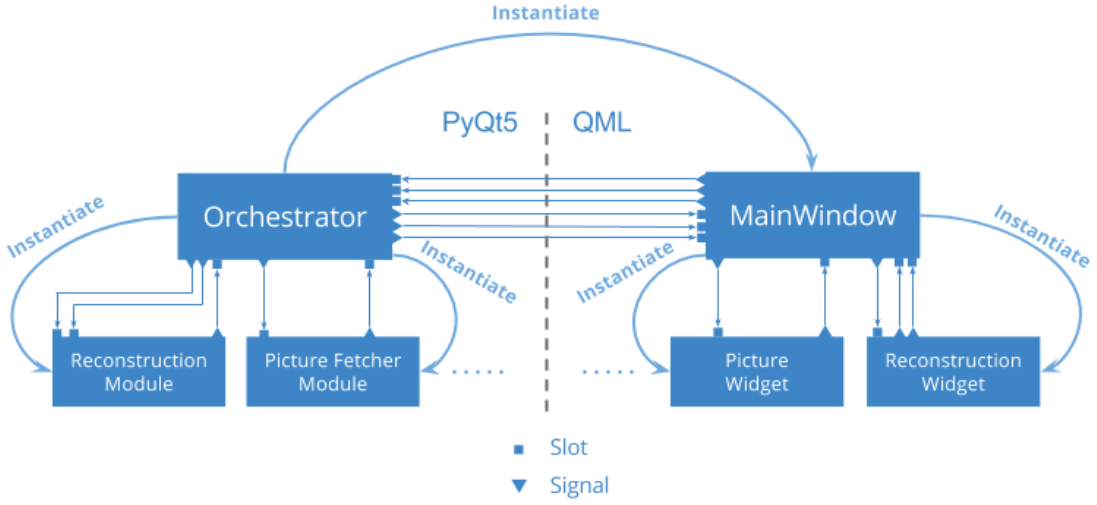
\includegraphics[width=\linewidth]{images/arch.png}
\caption{Architecture of the application (\texttt{PyQt5} for the model, \texttt{QML} for the view)}
\label{arch}
\vspace{-2mm}
\end{figure}


The last really important milestone we had was the 3D renderer : because python is more high level than C++, there are not really any optimised openGL libraries for python. But one important application requirement
was a performant renderer to render big point clouds. So instead of using openGL with python, we used openGL with C++ and then we created a QML plugin to import in PyQt. Though we first thought that this was a huge 
problem, it turns out to be a really good example on how our application was highly cutomizable and modular : one can easily import plugin coded in any language they want as long as they convert it into QML plugin. 